\documentclass[../../Thesis.tex]{subfiles}
\begin{document}
\header{Research results}
In this chapter the results of our research are presented; the detailed discussion on the meaning and implications of these results is presented in Chapter 6: Discussion.
\subheader{Ranking}
The Figures~\ref{figure:titleRanks} \&~\ref{figure:abstractRanks} show the result of the categorization task as ranking results. The rank indicates the position of the correct journal in the sorted list of matched journals. Figure~\ref{figure:titleRanks} shows the ranking results for the different sets based on the title. Figure~\ref{figure:abstractRanks} displays the ranking results based on the abstract. Both graphs show both average and median ranks, based on the cosine-similarity between the article and journal embeddings or feature vectors.
\clearpage
\begin{figure}[hbt]
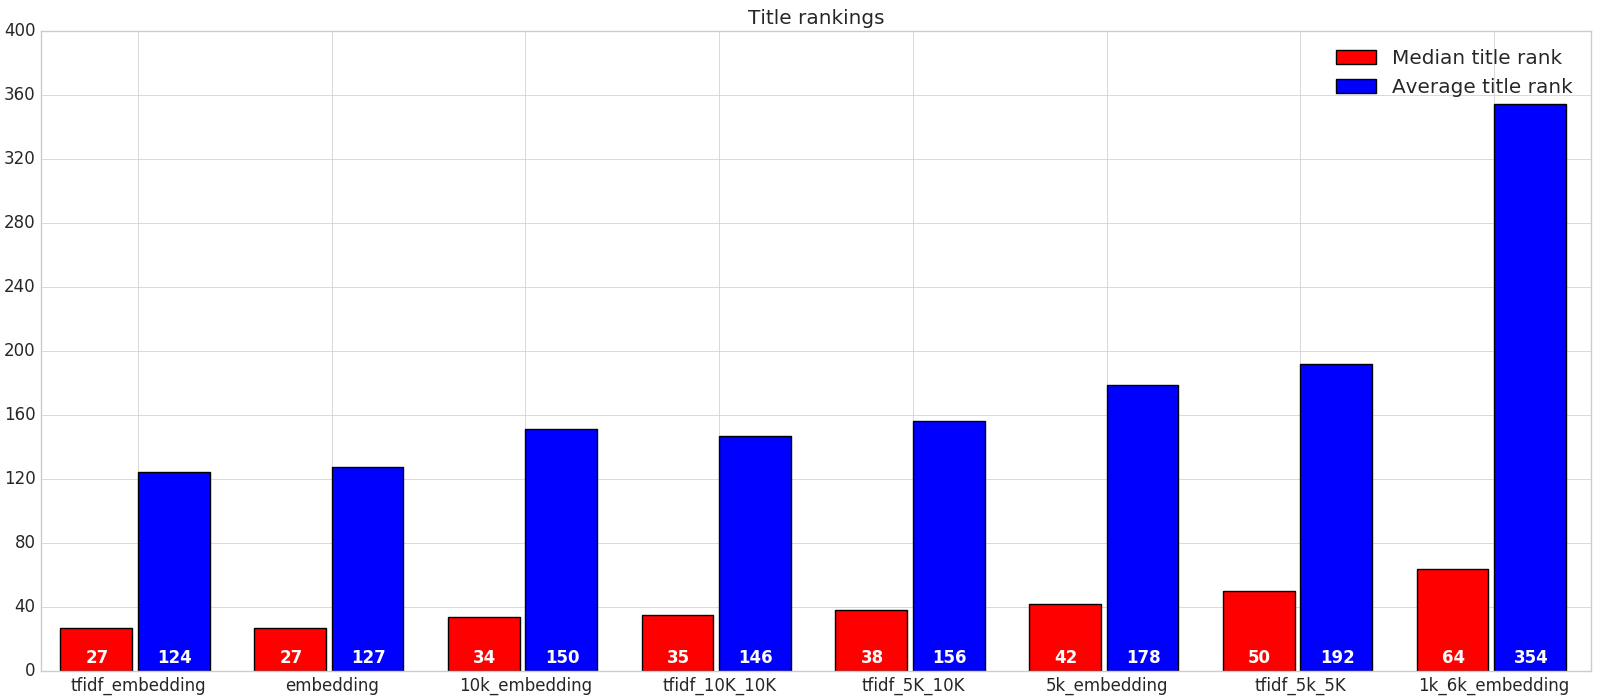
\includegraphics[width=6.5in]{Plots/Title_rankings}
\caption{Median and average title rankings}\label{figure:titleRanks}
\end{figure}
\begin{figure}[hbt]
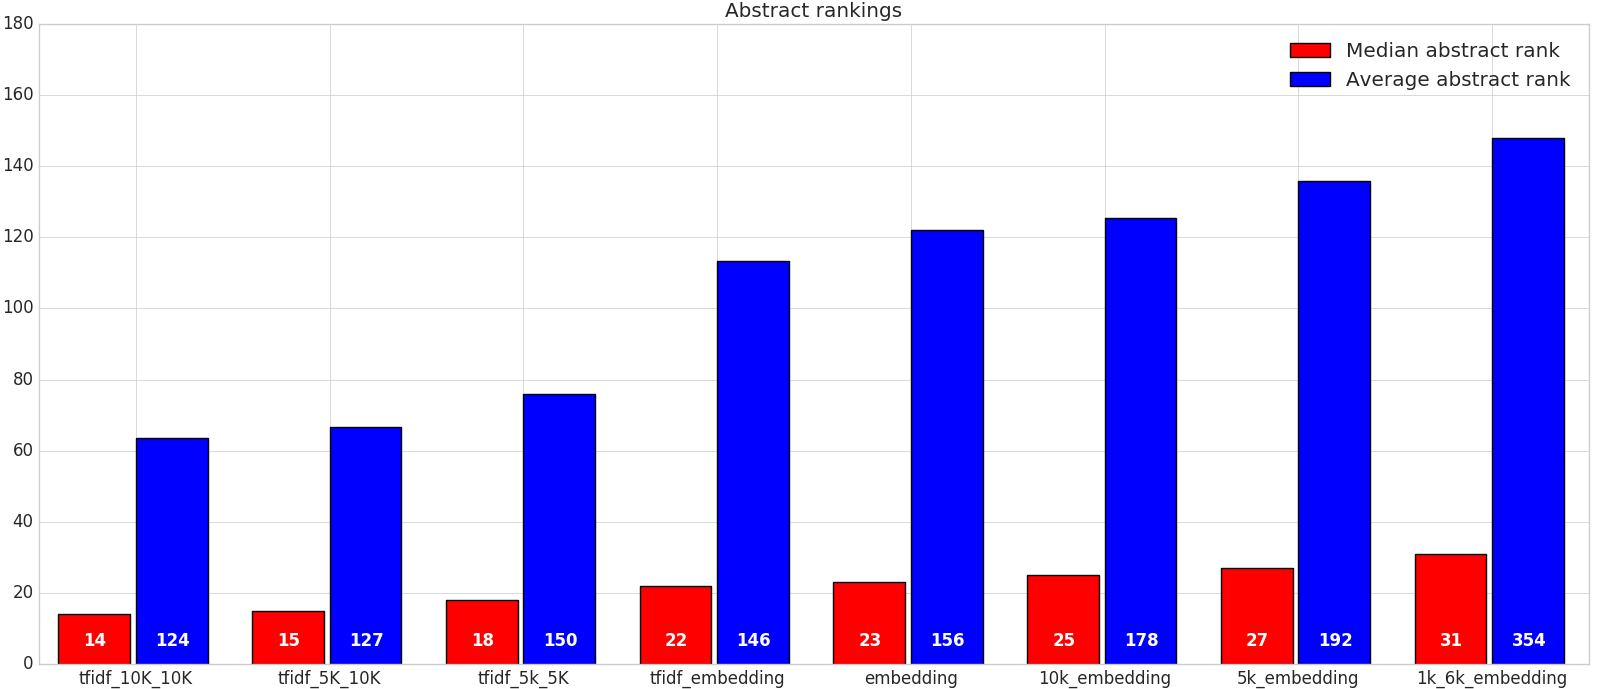
\includegraphics[width=6.5in]{Plots/Abstract_rankings}
\caption{Median and average abstract rankings}\label{figure:abstractRanks}
\end{figure}
\clearpage
\subheader{Rank distribution}
Figures~\ref{figure:titleDistribution} and~\ref{figure:abstractDistribution} show the distributions of the ranks for each set. The Figures plot the summed amount of articles against the ranks on a logarithmic scale. Figure~\ref{figure:titleDistribution} shows the rank distribution for the titles, Figure~\ref{figure:abstractDistribution} shows this for the ranks based on the abstract. These graphs give a detailed view of the ranks presented in their respective Figures~\ref{figure:titleRanks} and~\ref{figure:abstractRanks}. The Y-axis of the two Figures shows the fraction of the total number of articles. Due to this, all sets will have a maximum of 1. When 1 is hit, the graph stagnates since the dataset has reached the maximum fraction. The X-axis plots the ranks of the articles. These ranks are the ranks of each individual article in our validation set, in contrast to Figure~\ref{figure:titleRanks} and~\ref{figure:abstractRanks} which show average and median ranks.
\begin{figure}[hbt]
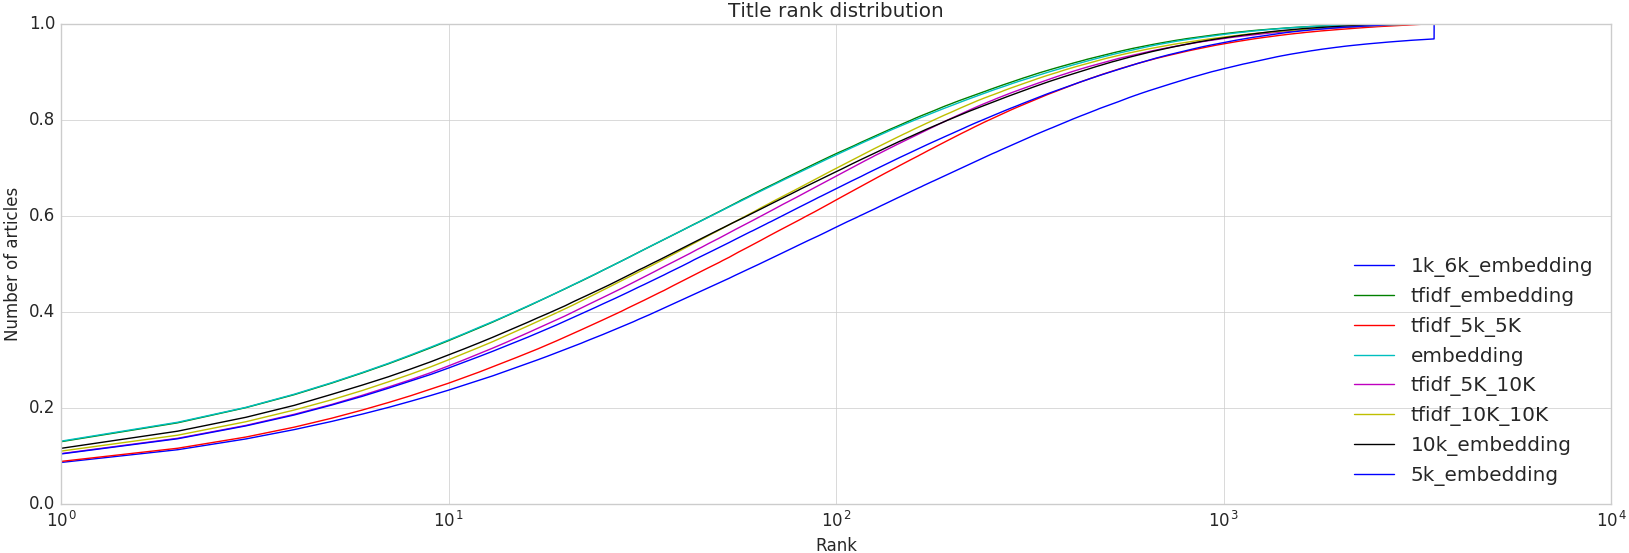
\includegraphics[width=6.5in]{Plots/Title_rank_distribution}
\caption{Title rank distribution per set}\label{figure:titleDistribution}
\end{figure}
\begin{figure}[hbt]
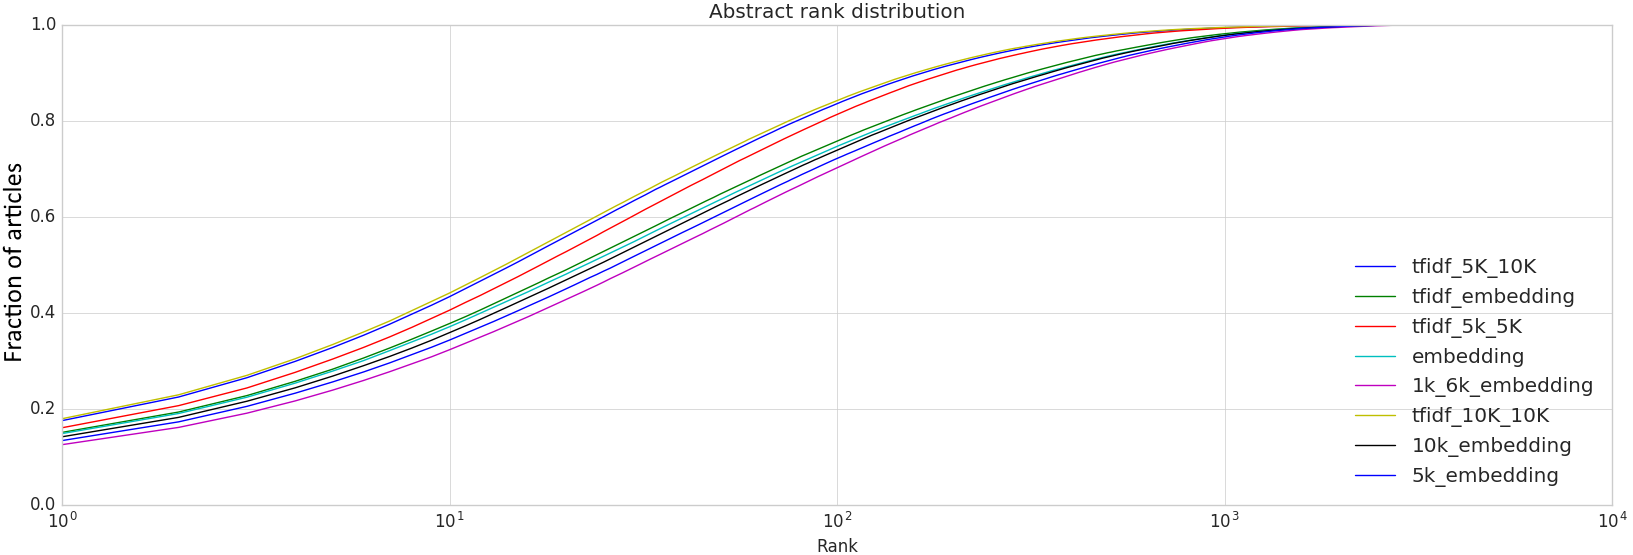
\includegraphics[width=6.5in]{Plots/Abstract_rank_distribution}
\caption{Abstract rank distribution per set}\label{figure:abstractDistribution}
\end{figure}

\clearpage
\subheader{F1-Score}
Figures~\ref{figure:f1Title} and~\ref{figure:f1Abstract} show the precision, recall and F1 scores. These scores are calculated on journal level, and are averaged per set. Figure~\ref{figure:f1Title} shows the F1 score for the title and Figure~\ref{figure:f1Abstract} shows the scores for the abstract. These scores indicate the performance of the sets on absolute hits/top-1. We show the precision and recall scores since they vary between sets that have similar F1-scores (i.e. Figure~\ref{figure:f1Title}, tfidf\_5k\_5k and tfidf\_embedding
\begin{figure}[hbt]
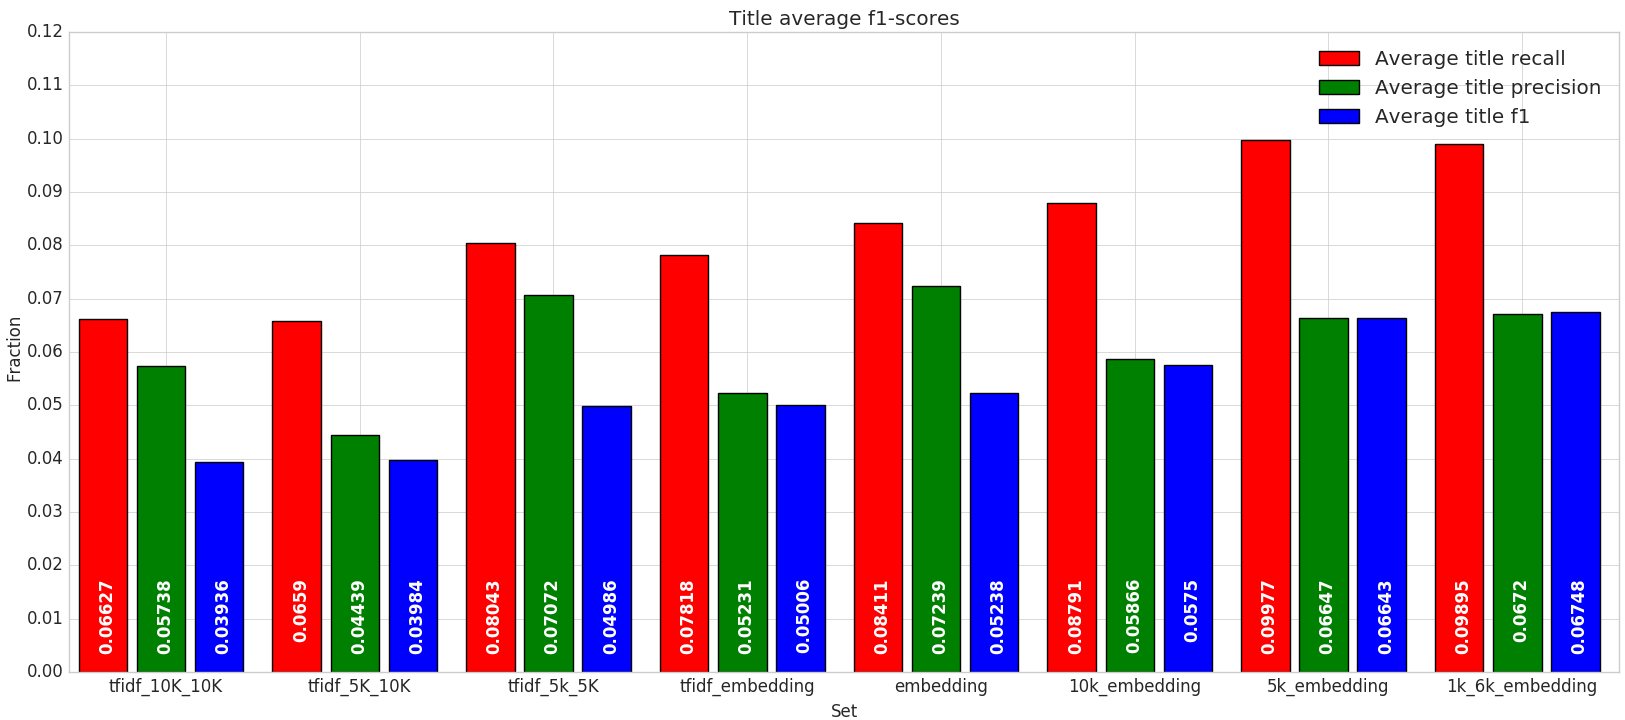
\includegraphics[width=6.5in]{Plots/Title_avg_f1}
\caption{Precision, recall and F1 scores based on title}\label{figure:f1Title}
\end{figure}
\begin{figure}[htb]
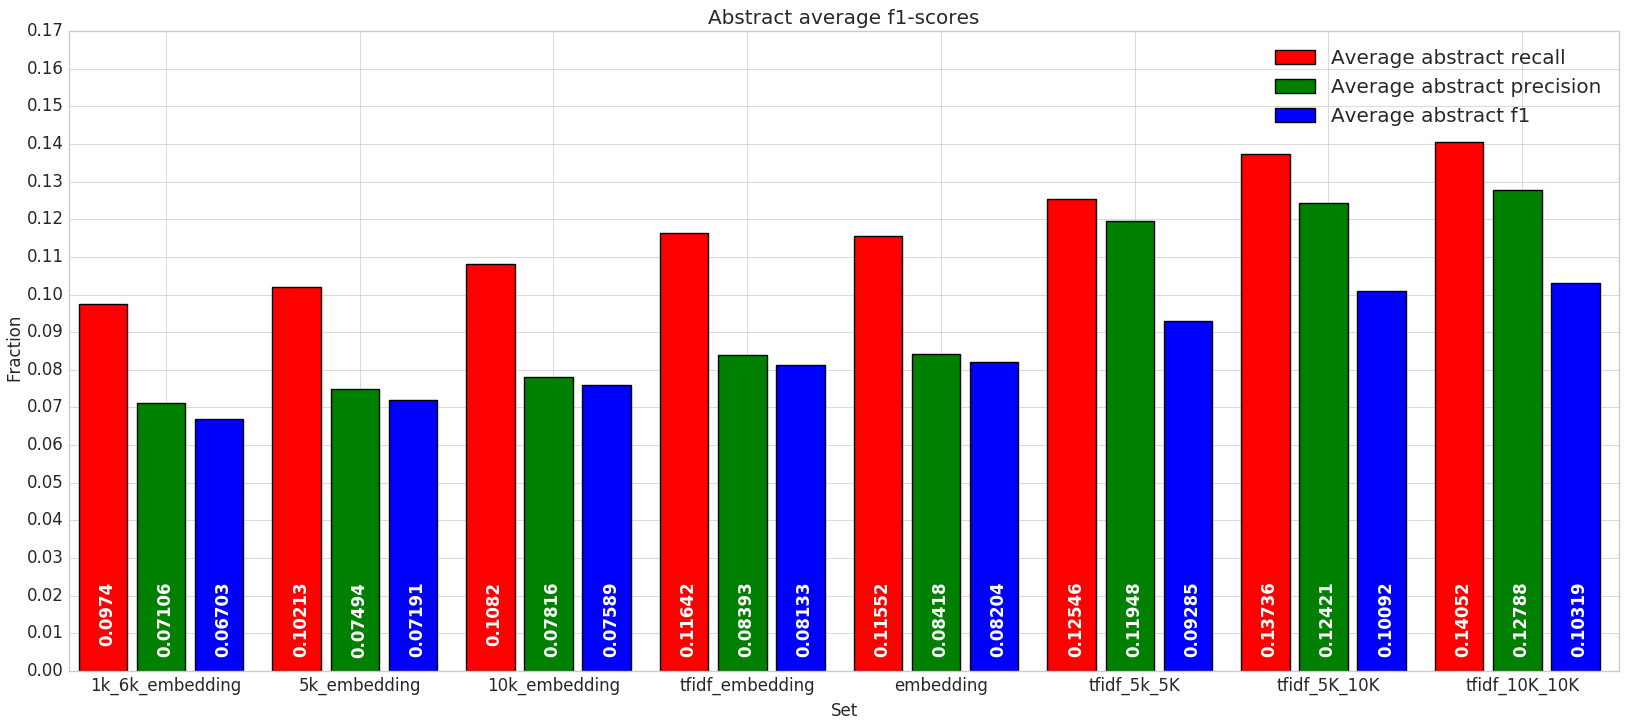
\includegraphics[width=6.5in]{Plots/Abstract_avg_f1}
\caption{Precision, recall and F1 scores based on abstract}\label{figure:f1Abstract}
\end{figure}
\clearpage
\subheader{Memory usage}
Table~\ref{table:memoryUsage} shows the total memory usage of each set for the \textit{Validation set}, indicating their storage costs in gigabytes\footnote{1024 based}. It furthermore shows the absolute hit percentage of the title and the abstracts, i.e. the percentage of articles that have their source\footnote{Journal from which the article was taken} journal as the first result in the ranking. The table furthermore shows the median rank and the median abstract rank, as visualized in Figures \ref{figure:titleRanks} and~\ref{figure:abstractRanks}. Thus, this table gives an overview of the memory usage of the sets, combined with their performance on the ranking task.\\
\begin{table}[hbt]
\begin{center}
\begin{tabular}{|l|r|r|r|r|}
\hline
Set & Size in GB & Absolute hit percentage & Median title rank & Median abstract rank\\
&&\begin{tabular}{p{0.5in}|p{0.5in}}Title & Abstract\end{tabular}&&\\
\hline
tfidf 5k 5K & $9.82$ & \begin{tabular}{p{0.5in}|p{0.5in}}5.42\% & 10.18\%\end{tabular} & 50 & 27\\
\hline
tfidf 5K 10K & $11.47$ & \begin{tabular}{p{0.5in}|p{0.5in}}6.49\% & 11.08\%\end{tabular} & 38 & 15\\
\hline
\textbf{tfidf 10K 10K} &\textbf{11.61}& \begin{tabular}{p{0.5in}|p{0.5in}}\textbf{6.79\%} & \textbf{11.32\%}\end{tabular} & \textbf{35} & \textbf{14}\\
\hline
embedding & $3.13$ & \begin{tabular}{p{0.5in}|p{0.5in}}7.92\% & 9.24\%\end{tabular} & 27 & 23\\
\hline
5k embedding & $3.13$ & \begin{tabular}{p{0.5in}|p{0.5in}}6.34\% & 8.36\%\end{tabular} & 42 & 27\\
\hline
10k embedding & $3.13$ & \begin{tabular}{p{0.5in}|p{0.5in}}7.03\% & 8.76\%\end{tabular} & 34 & 25\\
\hline
\textbf{tfidf embedding} & \textbf{3.13} & \begin{tabular}{p{0.5in}|p{0.5in}}\textbf{7.89\%} & \textbf{9.33\%}\end{tabular} & \textbf{27} & \textbf{22}\\
\hline
1k 6k embedding & $3.06$ & \begin{tabular}{p{0.5in}|p{0.5in}}5.16\% & 7.86\%\end{tabular} & 64 &31 \\
\hline
\end{tabular}
\end{center}
\caption{Memory usage and performance for each set}\label{table:memoryUsage}
\end{table}
\subheader{Journal relatedness plot}
We created four seperate journal plots, Figures~\ref{figure:titlePlotNormal} and~\ref{figure:titlePlotGrouped} show the title based embeddings, and Figures~\ref{figure:abstractPlotNormal} and~\ref{figure:abstractPlotGrouped} show the abstract based embeddings.
Figures~\ref{figure:titlePlotNormal} and~\ref{figure:abstractPlotNormal} show the two dimensional plots of the journal embeddings. The journals are color-marked by publisher. Red is Wiley, lime is Elsevier and blue is Springer Nature. The grey points are other or not-specified publishers.
Figures~\ref{figure:titlePlotGrouped} and~\ref{figure:abstractPlotGrouped} show the journal embeddings grouped by a k-means algorithm, creating 8 groups. The bottom right of the plot shows the names of the journals closest to the center of the group. While most names state the topic of the research field, two do not. These are \textit{RSC Advances}: chemical sciences, and \textit{Symmetry}:  research on symmetry phenomena wherever they occur in mathematical or scientific studies. The k-means algorithm ran on the 300-dimensional vectors, while the plot shows the 2-dimensional vectors. In the title-based Figures (\ref{figure:titlePlotNormal} \&~\ref{figure:titlePlotGrouped}) the journals \textit{PNAS} and \textit{Cell} overlap each others labels on the bottom right side of the graph. In the abstract-based Figures (\ref{figure:abstractPlotNormal} \&~\ref{figure:abstractPlotGrouped}) the journals \textit{PNAS} and \textit{Nature} overlap each others label on the bottom right side of the graph.
The digital versions of these plots can be found at:~\url{https://goo.gl/nCGMcu} (title-based) and~\url{https://goo.gl/LwYP6k} (abstract-based). The usage of this digital version is advised, since this interactive plot enables zooming and adjusting plot settings, which can give a broader insight into the results than the presented figures. Although the presented figures give sufficient insight for the purpose of this thesis.
\begin{landscape}
\begin{figure}
\begin{center}
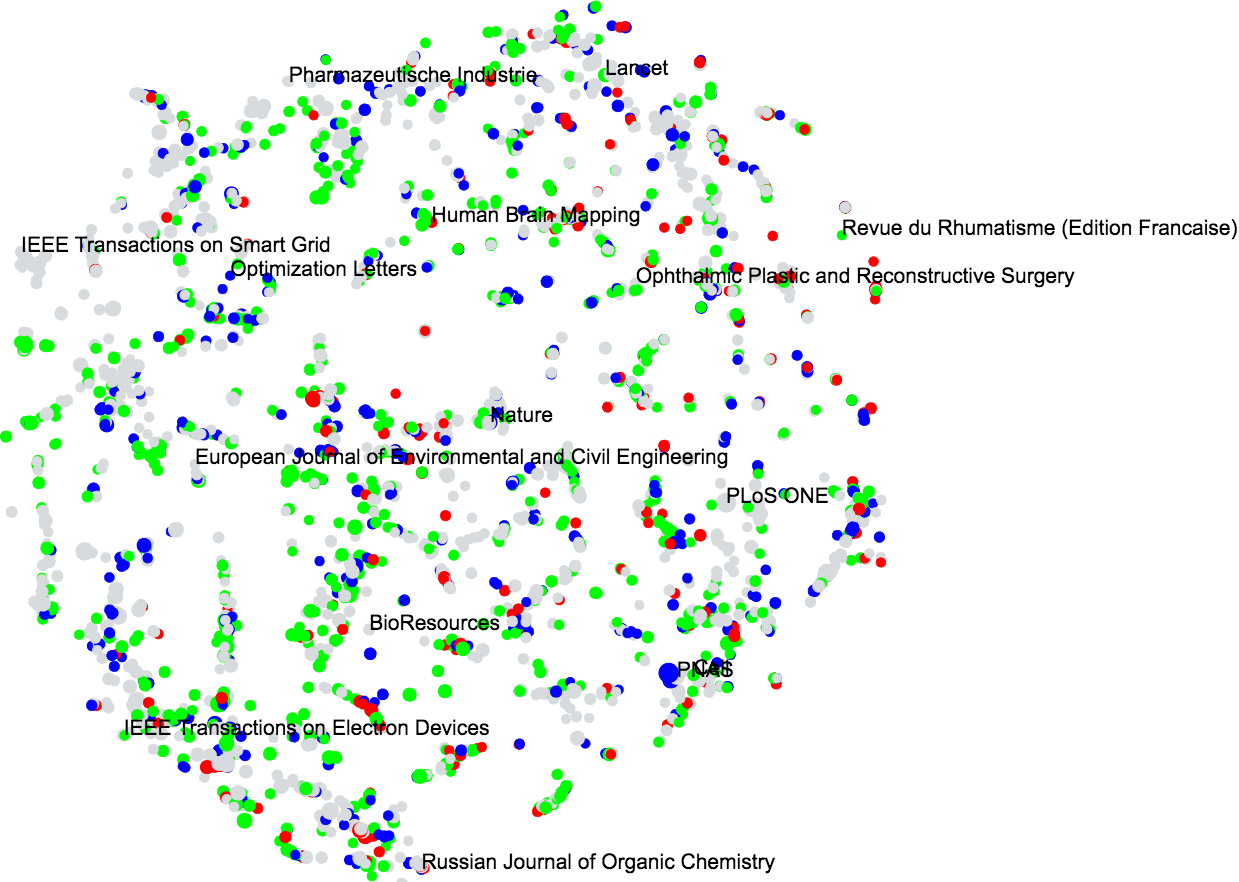
\includegraphics[height=6.5in]{Plots/Journal_Plots/Title_normal}
\end{center}
\caption{Journal plot of title embeddings, grouped by publisher}\label{figure:titlePlotNormal}
\end{figure}
\end{landscape}

\begin{landscape}
\begin{figure}
\begin{center}
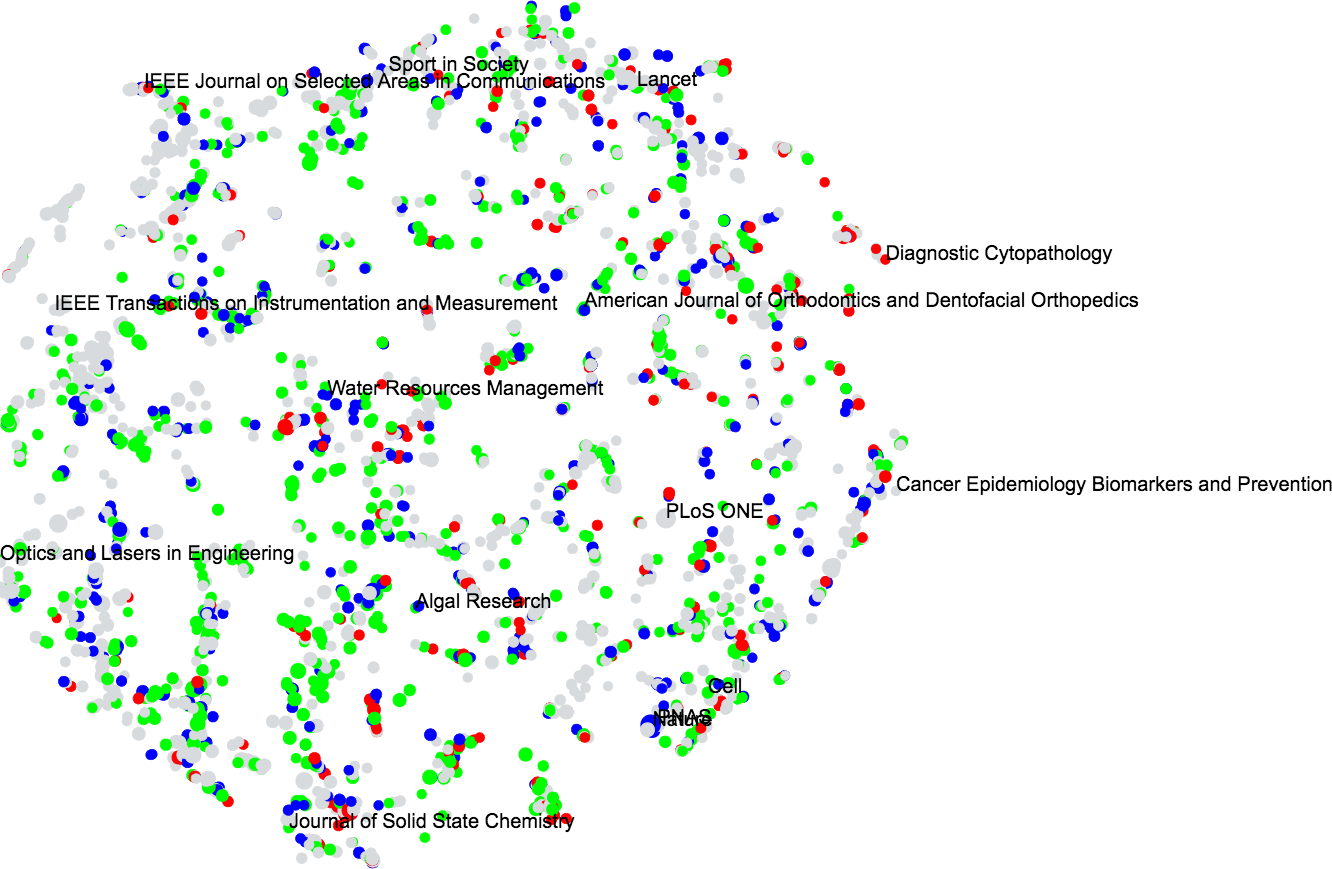
\includegraphics[height=6.5in]{Plots/Journal_Plots/Abstract_normal}
\end{center}
\caption{Journal plot of abstract embeddings, grouped by publisher}\label{figure:abstractPlotNormal}
\end{figure}
\end{landscape}

\begin{landscape}
\begin{figure}
\begin{center}
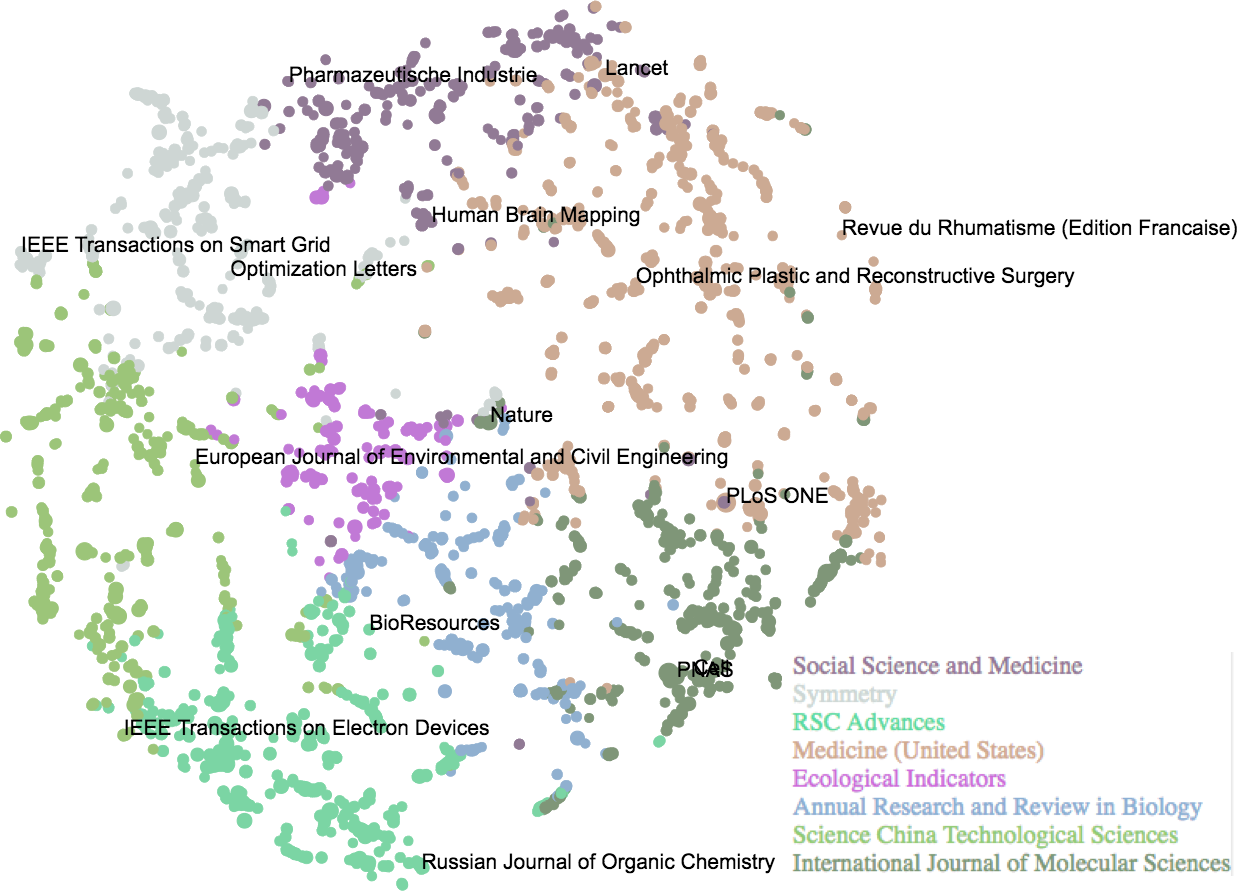
\includegraphics[height=6.5in]{Plots/Journal_Plots/Title_grouped}
\end{center}
\caption{Journal plot of title embeddings, k-means grouped}\label{figure:titlePlotGrouped}
\end{figure}
\end{landscape}

\begin{landscape}
\begin{figure}
\begin{center}
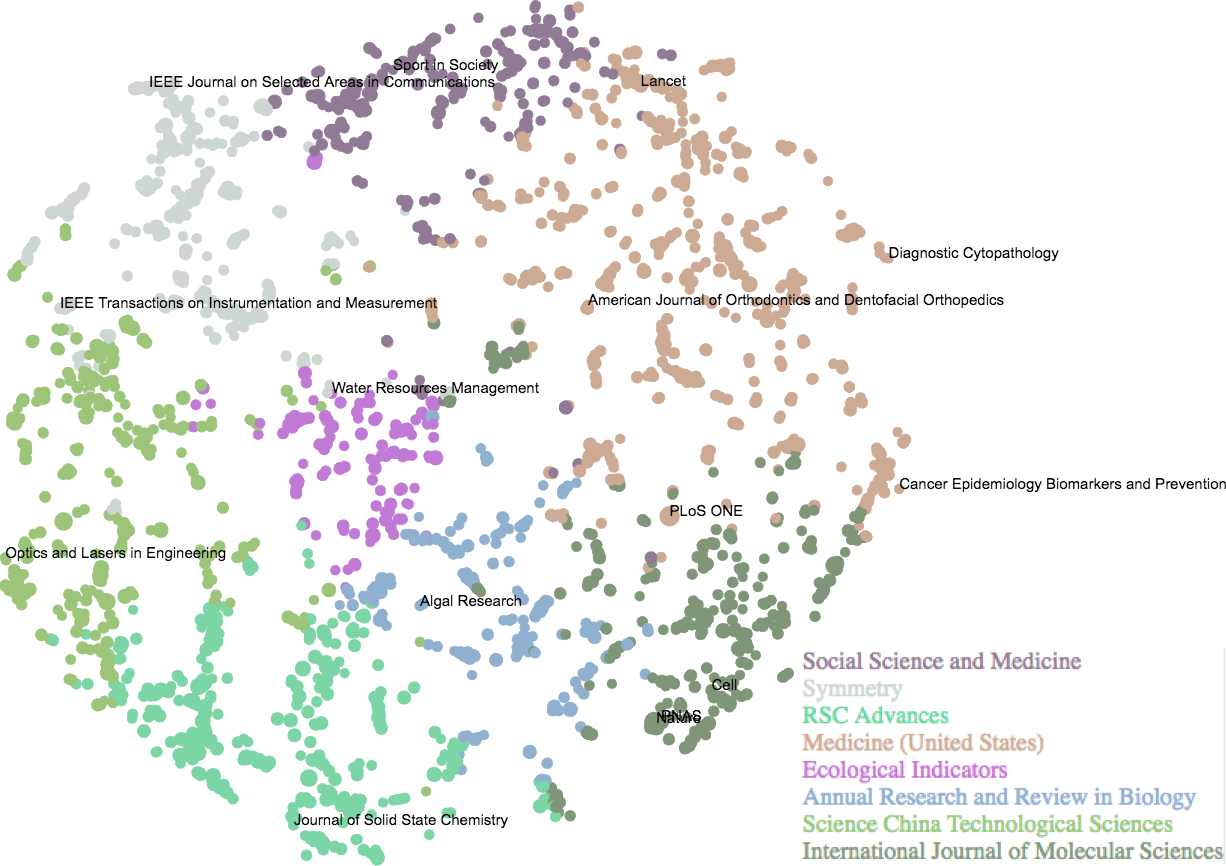
\includegraphics[height=6.5in]{Plots/Journal_Plots/Abstract_grouped}
\end{center}
\caption{Journal plot of abstract embeddings, k-means grouped}\label{figure:abstractPlotGrouped}
\end{figure}
\end{landscape}
\end{document}